To evaluate the performance of our DiffTrack algorithm, we conducted two quantitative evaluations using real code revision data obtained from open source repositories on GitHub.
We have two objectives for our evaluations: 1) to quantify how accurately the algorithm can estimate a code piece; and 2) to quantify how accurately the algorithm can extract a set of commits given a code piece.
%We here report our experimental design and results.

\subsection{Code Piece Matching Accuracy}

%\subsubsection{Dataset}

\begin{table}[tbp]
	\centering
	\begin{tabular}{ c c c }
	   \small\textit{Repository Name} & \small\textit{\#Pull Requests} & \small\textit{\#Contributors} \\
       \midrule
		mailtrain & 24 & 9 \\
      portainer & 212 & 47 \\
      styletron & 32 & 9 \\
      claudia & 35 & 13 \\
      Chart.js & 1064 & 201 \\
	\end{tabular}
    \caption{Open source repositories used in our code piece matching accuracy evaluation.}
	\label{table:repositories}
\end{table}

% \begin{table}
%   \centering
%   \begin{tabular}{l r r r}
%     % \toprule
%     & & \multicolumn{2}{c}{\small{\textbf{Test Conditions}}} \\
%     \cmidrule(r){3-4}
%     {\small\textit{Name}}
%     & {\small \textit{First}}
%       & {\small \textit{Second}}
%     & {\small \textit{Final}} \\
%     \midrule
%     Marsden & 223.0 & 44 & 432,321 \\
%     Nass & 22.2 & 16 & 234,333 \\
%     Borriello & 22.9 & 11 & 93,123 \\
%     Karat & 34.9 & 2200 & 103,322 \\
%     % \bottomrule
%   \end{tabular}
%   \caption{Table captions should be placed below the table. We
%     recommend table lines be 1 point, 25\% black. Minimize use of
%     table grid lines.}~\label{tab:table1}
% \end{table}


% \begin{figure*}
%   \centering
%   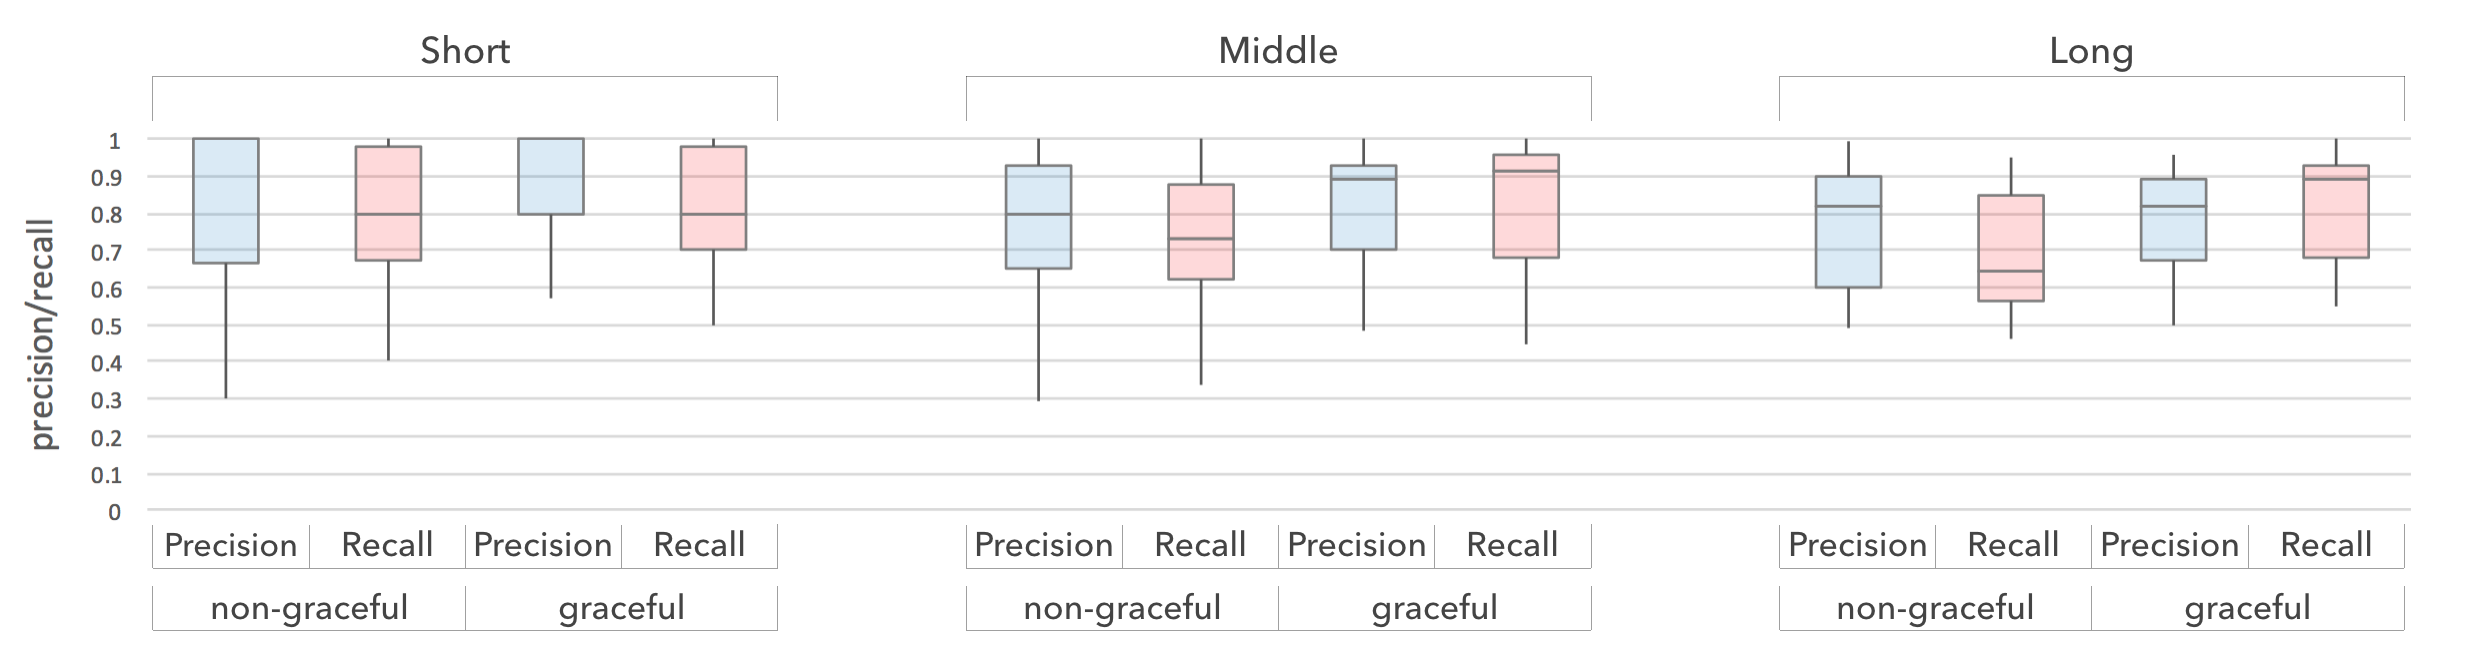
\includegraphics[width=2.0\columnwidth]{evaluate/difftrack_eval_commit.png}
%   \caption{Box plots of DiffTrack commit matching accuracy performance results.}~\label{fig:Commit_Matching_Accuracy_Evaluation}
%   \vspace{-5mm}
% \end{figure*}

We searched publicly-available repositories on GitHub that satisfied the following criteria:

\begin{itemize}
\setlength{\itemsep}{0cm}
\item A repository was active as of February 2017.
\item Multiple developers were involved.
\item Developers actively used pull requests and wrote review comments.
\item A repository was marked as favorite by over 1000 people.
\end{itemize}

As a result, we selected five repositories as summarized in Table~\ref{table:repositories}.
We then extracted commits from these repositories and manually checked them to remove minor revisions (e.g., fixing a typo) from this evaluation.
In addition, we chose commits where a knowledgeable person can easily identify a pair of code pieces between the two versions.
This process resulted in 180 commits.
After annotating ground truth data through manual labeling, we classified the collected commits into nine group (20 commits in each) in terms of the following two factors:

\begin{itemize}
\setlength{\itemsep}{0cm}
\item The types of changes included (\textit{Type}): \textit{Add} (only additions); \textit{Del} (only deletions); and \textit{AddDel} (both).
\item The number of lines changed (\textit{Length}): \textit{Short} ($\sim 9$ lines); \textit{Medium} ($10 \sim 30$ lines); and \textit{Long} ($30 \sim$ lines).
\end{itemize}

\textit{AddDel} represents cases of an update (i.e., lines in a code piece were replaced); a move (i.e., the location of a code piece was changed); a combination of both; and refactoring.
Thus, \textit{AddDel} generally represents difficult test cases for DiffTrack to accurately estimate a target code piece. 


\begin{table}[t]
    \centering
    \label{my-label}
    \begin{tabular}{cc||c|c| c}
                                                  &  & \textit{Add}           & \textit{Del}           & \textit{AddDel}        \\ \hline \hline 
\multirow{2}{*}{\textit{Short}}                     & $P_{cp}$ & 1.00 (0.00) & 0.95 (0.22) & 0.88 (0.31) \\
& $R_{cp}$ & 0.99 (0.05) & 0.95 (0.22) & 0.83 (0.32) \\ \hline
%& $F_{cp}$ & 0.99 (0.03) & 0.95 \koji{(0.95)}{} & 0.85 (0.31) \\ \hline
\multirow{2}{*}{\textit{Middle}}
& $P_{cp}$ & 0.94 (0.22) & 0.95 (0.22) & 0.96 (0.10)  \\
& $R_{cp}$ & 0.95 (0.22) & 0.95 (0.22) & 0.89 (0.15) \\ \hline
%& $F_{cp}$ & 0.95 (0.22) & 0.95 (0.22) & 0.91 (0.10)  \\ \hline
\multirow{2}{*}{\textit{Long}}
& $P_{cp}$ & 0.99 (0.06) & 0.90 (0.31) & 0.93 (0.23) \\
& $R_{cp}$ & 1.00 (0.00) & 0.90 (0.31) & 0.87 (0.23) \\
%& $F_{cp}$ & 0.99 (0.03) & 0.90 (0.31) & 0.89 (0.22)
    \end{tabular}
    \caption{Accuracy performance of code piece matching across the nine groups. $P_{cp}$ and $R_{cp}$ represent precision and recall, respectively. Values in parentheses represent the standard deviations.}
    \label{table:performance}
    \vspace{-2mm}
\end{table}




\subsubsection{Results}
Table \ref{table:performance} shows the performance of the algorithm across the nine categories.
We used the precision and recall ($P_{cp}$, $R_{cp}$) to evaluate the accuracy of estimated code pieces.
More specifically, $P_{cp} = \frac{l_c}{l_c + l_i},\;\; R_{cp} = \frac{l_c}{l_c + l_n},$ where $l_c$, $l_i$, and $l_n$ represent the numbers of lines correctly included in $\widehat{CP_{T}}$, lines incorrectly included in $\widehat{CP_{T}}$, and lines $CP_{T}$ that are not included in $\widehat{CP_{T}}$, respectively.

% \vspace{-4mm}
% \begin{equation*}
% P_{cp} = \frac{l_c}{l_c + l_i},\;\; R_{cp} = \frac{l_c}{l_c + l_n}, 
% \end{equation*}


Overall, DiffTrack exhibited high precision and recall regardless of the length of code pieces and types of revisions.
In particular, it identified code pieces almost perfectly when revisions included only additions.
Changes in \textit{AddDel} were the most difficult case, but DiffTrack was still able to identify target code pieces at reasonable precision and recall.
An evaluation on GumTree found that it was able to identify move operations accurately~\cite{GumTree} (although it is not designed to backtrack changes on code pieces as we already discussed).
Our results show that DiffTrack performs well in a wider variety of \textit{AddDel} cases, including updates, combinations of moves and updates, and refactoring.
We thus concluded that code piece matching in DiffTrack demonstrates sufficient robustness for our purpose.



\subsection{Commit Matching Accuracy Evaluation}
%\subsubsection{Dataset}
We evaluated the accuracy of selected commits by DiffTrack.
We chose  100 code pieces (34 \textit{Short}, 33 \textit{Middle}, and 33 \textit{Long}) from the Chart.js repository.
We then manually traced back the development history, and created the ground truth data consisting of more than five commits associated with each original source code piece.


\subsubsection{Results}
We used precision and recall for this evaluation.
The definitions of these metrics are the same as those for the code piece matching performance evaluation except using the number of commits.
Figure~\ref{fig:Commit_Matching_Accuracy_Evaluation} shows the performance of the algorithm.
Overall accuracy performance was high regardless across the conditions.
We ran multi-level linear regression analysis with two factors: \textit{Length} and the presence of graceful matching.
The result showed that graceful matching significantly improved precision and recall.
The estimated coefficients were 0.058 ($SE=0.025$, $p<0.05$) and 0.051 ($SE=0.021$, $p<0.05$) for precision and recall, respectively.
\textit{Short} also showed significantly higher precision and recall than \textit{Long} ($p<0.05$).


The results suggest that our graceful approach can improve precision and recall of identifying commits by roughly 5\% in our dataset.
Although the effect estimated by our multi-level linear regression was not large, it offers robustness to cases in which the default DiffTrack algorithm exhibits low precision and recall as shown in Figure~\ref{fig:Commit_Matching_Accuracy_Evaluation}.
In one test case, the na\"{i}ve DiffTrack algorithm was only able to achieve the precision and recall of 0.30 and 0.40, respectively, but the graceful approach improved both of them to 0.80.
We thus concluded that the graceful approach can improve commit matching and should be included in the CodeGlass system.
